\chapter{Laboratorio 4}

Il primo circuito analizzato è il multivibratore monostabile (\Fig\ref{fig:circuito_1}). Tale circuito presenta uno stato stabile, in cui rimane fino a che un impulso esterno di comando lo porta in un secondo stato, in cui il circuito rimane per un tempo predefinito per poi tornare spontaneamente nello stato stabile, in attesa di un successivo impulso.
\begin{figure}[h]
	\centering
	\begin{minipage}{.45\textwidth}
		\scalebox{.62}{
			\begin{circuitikz}
				\draw (2,6) node[op amp, anchor=-](oa){\texttt{TL071}};
				\draw (oa.-) -- ++(-2, 0) coordinate (D) -- ++(-2,0) to[C=$C$] ++(0,-1.5) node[ground]{};
				\draw (D) to[D=$D$] ++(0,-1.5) node[ground]{};
				\draw (oa.up) -- ++(0, 0.3) node[vcc]{$V_{DD}$};
				\draw (oa.down) -- ++(0,-0.3) node[vee]{$V_{SS}$};
				\draw (oa.out) -- ++(1,0) coordinate(loop);
				\draw (loop) -- ++(0,-2.3) coordinate(R2) to[R=$R_2$] ++(-3.39,0) coordinate(rg) (R2-|oa.+) -- (oa.+);
				\draw (oa.-) -- ++(0,1.7) to[R=$R_3$]++(3.39,0) coordinate(Rf) (Rf-|loop) -- (loop);
				\draw (oa.+) to[short, -o] ++(0,0) ++(-.1,0) node[left]{$v_+$};
				\draw (oa.-) to[short, -o] ++(0,0) ++(0,-.1) node[below]{$v_-$};
				\draw (rg) -- ++(-1,0) coordinate(r1) to[R=$R_1$] ++(0,-2) node[ground]{};
				\draw (r1) to[D=$D_T$] ++(-2.5,0) coordinate(vt) to[C=$C_T$] ++(-3,0) coordinate(vin);
				\draw (vt) to[R=$R_T$] ++(0,-2) node[ground]{};
				\draw (vt) to[short, -o] ++(0,0) node[above]{$v_t$};
				\draw (loop) to[short, -o] ++(0,0) ++(.1,0) node[right]{$v_{out}$};
				\draw (vin) to[sV=$v_{in}$] ++(0,-2) node[ground]{};
				\draw[thick] (-5.5,0) rectangle (6.5,8.5);
			\end{circuitikz} 
		}
	\end{minipage}\qquad
	\begin{minipage}{.45\textwidth}
		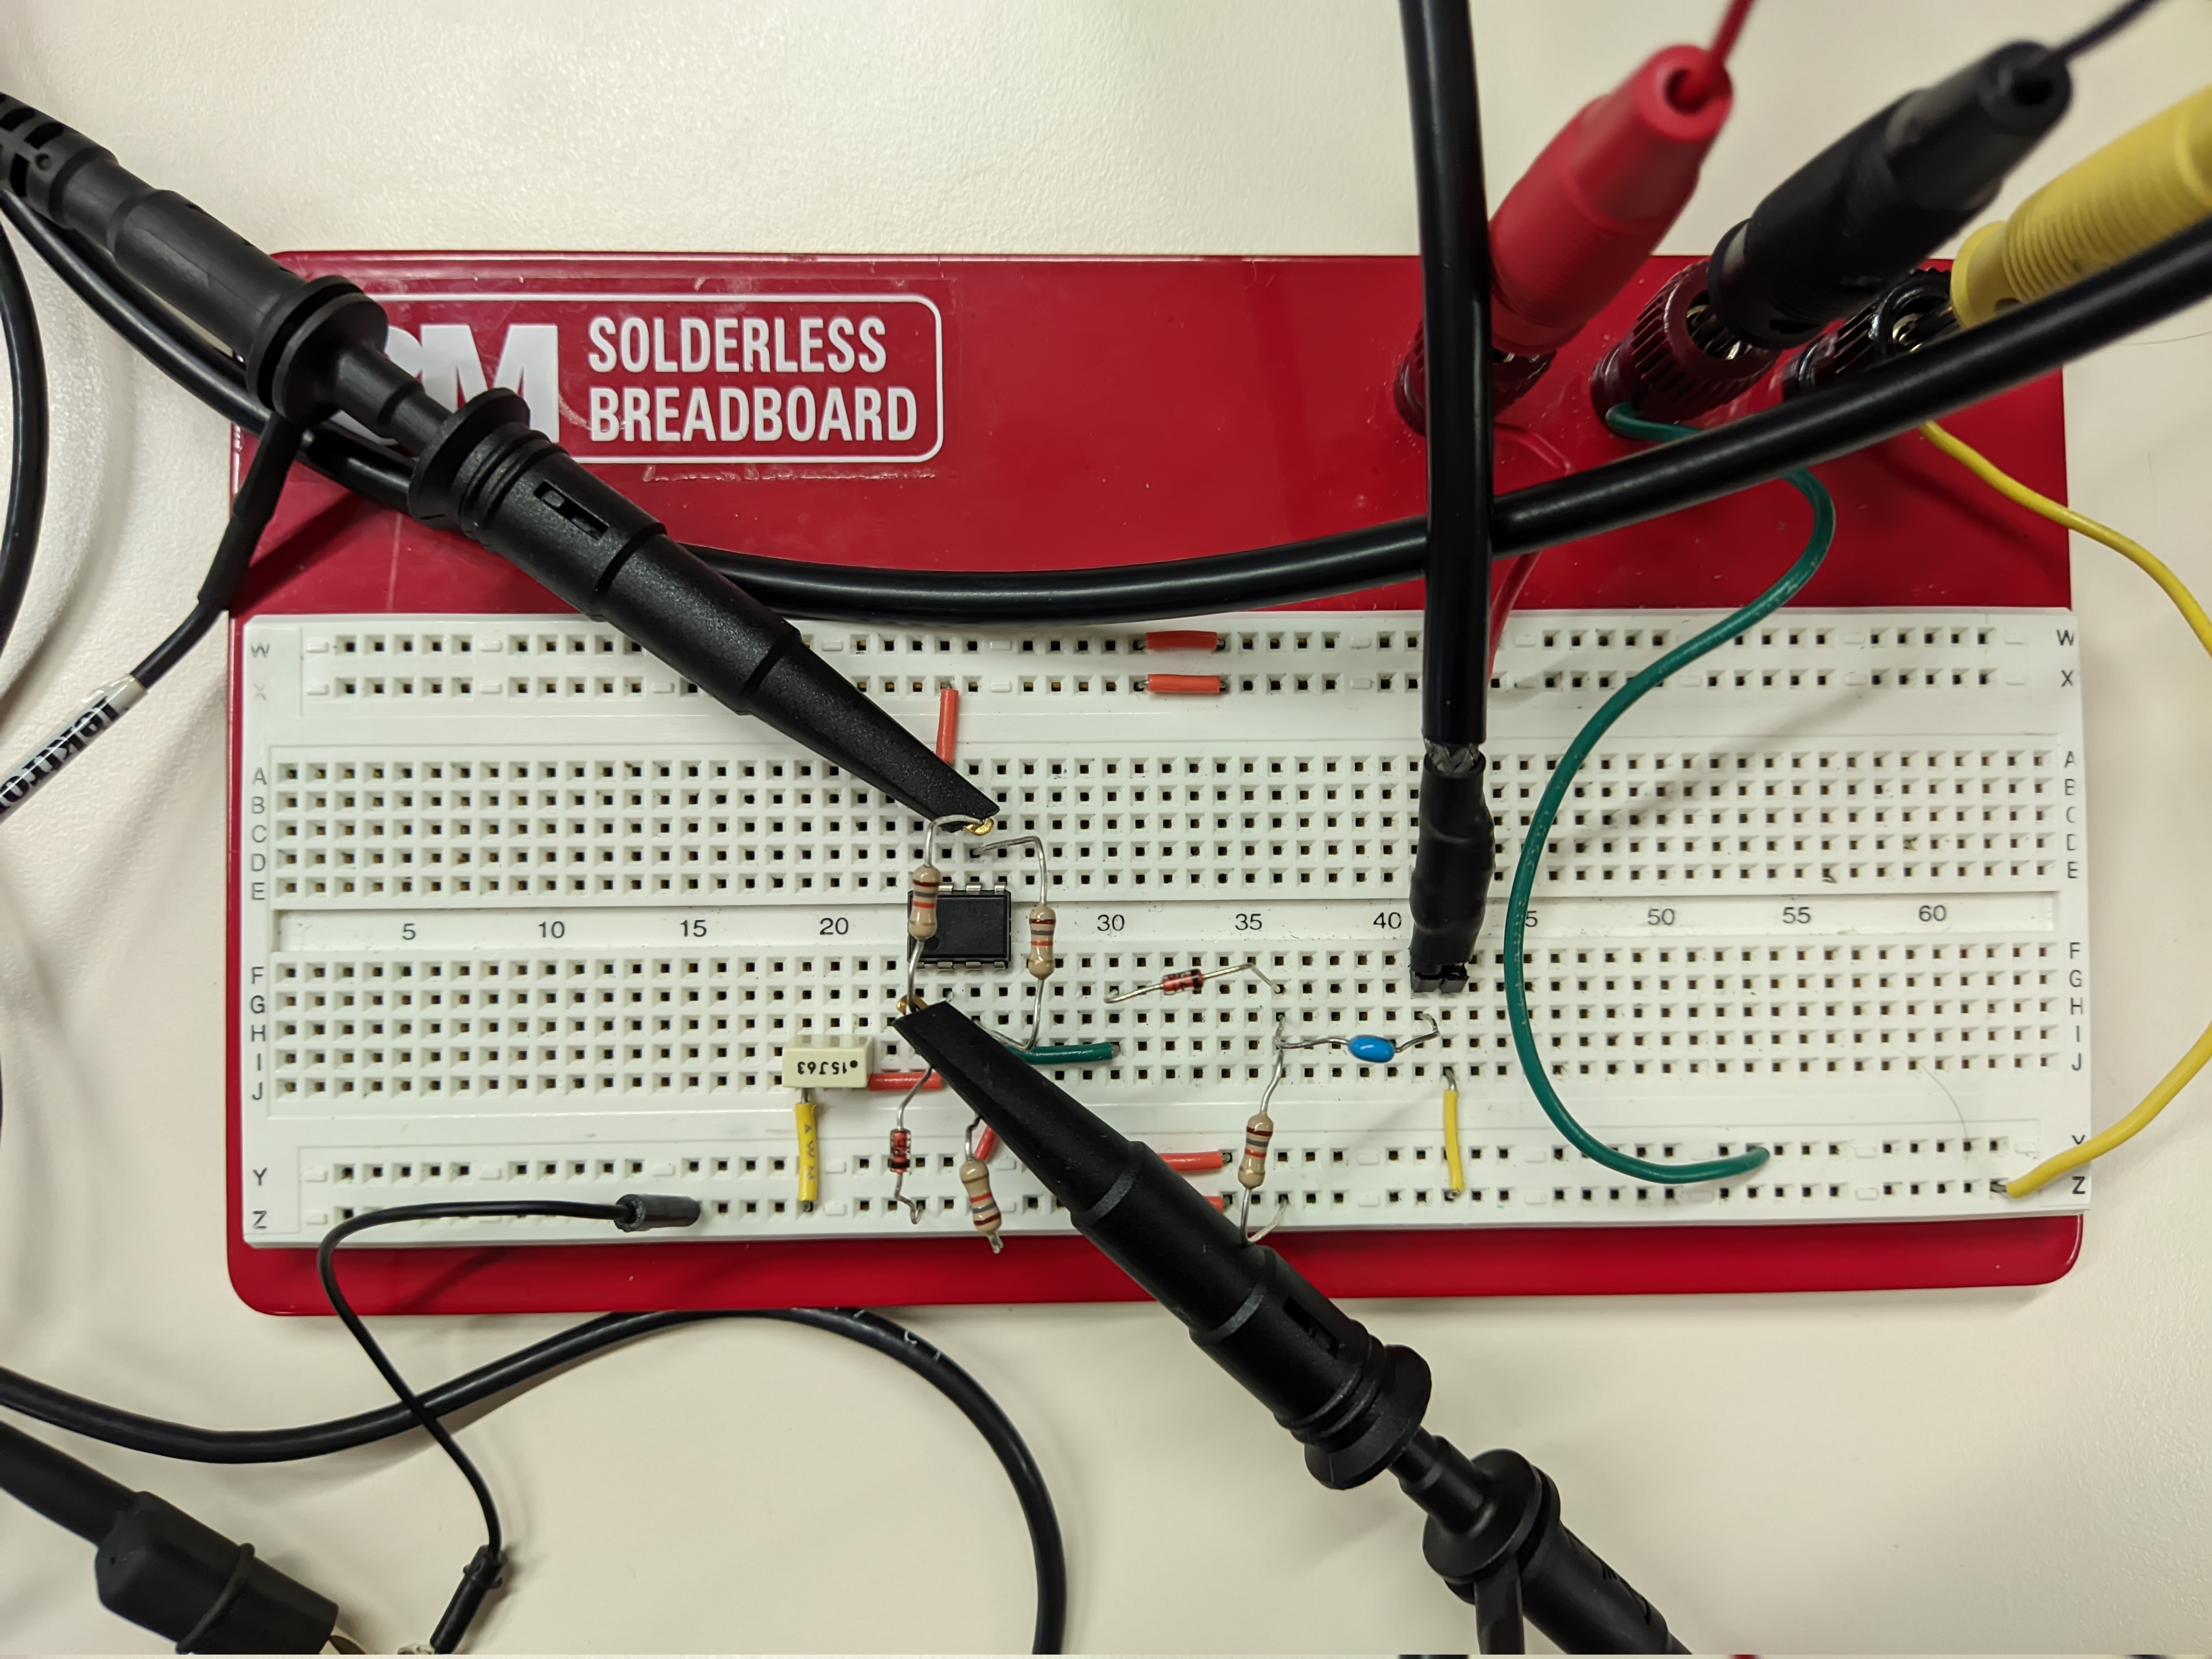
\includegraphics[width=\linewidth]{./ImageFiles/Laboratorio 4/CIR11.jpg}
	\end{minipage}
	\caption{Schema circuitale del multivibratore monostabile e foto del circuito realizzato.}
	\label{fig:circuito_1}
\end{figure}
A livello costruttivo si parte dal generatore d'onda quadra visto nello scorso laboratorio: inserendo un diodo $D$ in parallelo alla capacità $C$ si ottiene uno stato stabile. In questo caso, quando la tensione di uscita è pari a $v_{out}>0$ la capacità si carica, ma quando la tensione ai capi del condensatore raggiunge circa $0.7V$ (tensione di polarizzazione del diodo $D$) smette di caricarsi perché il diodo offre un cortocircuito per la corrente fornita dall'amplificatore. 

\noindent
Poiché il circuito commuti dallo stato stabile $v_{out}=V_{DD}$ allo stato quasi stabile $v_{out}=V_{SS}$ è necessario che la tensione dell'ingresso non invertente scenda al di sotto della tensione applicata all'ingresso invertente. Questo è possibile tramite l'applicazione sul morsetto non invertente di un picco di tensione negativo. Per fare ciò si inserisce un circuito derivatore composto da una capacità $C_T$ ed una resistenza $R_T$. Tale circuito ha il compito di generare, a partire da un segnale rettangolare $v_in$, un impulso negativo ed uno positivo. Poi, grazie all'inserimento del diodo $D_T$, l'unico impulso presentato al morsetto non invertente è quello negativo. 

\noindent
Questo impulso negativo porterà per un breve istante la tensione $v_+$ al di sotto della tensione presente ai capi del condensatore (che è pari alla tensione di polarizzazione del diodo) forzando la commutazione dell'uscita a $v_{out}=V_{SS}$. A questo punto, il condensatore si scarica fino a raggiungere la tensione di soglia $V_H^-$ e una volta raggiunta la tensione di soglia cambia nuovamente e l'uscita commuta portandosi a $v_{out}=V_{DD}$. Il condensatore ricomincia così il ciclo di carica ma una volta raggiunta la tensione di polarizzazione del diodo si blocca e il circuito entra di nuovo in uno stato stabile in attesa che sul morsetto non invertente venga generato un impulso negativo. Il tempo per cui $v_{out}=V_{SS}$ dipende dalla capacità $C$ e dalla resistenza $R3$.

I valori utilizzati nel circuito sono indicati nella tabella \ref{tab:valori_componenti_1}. L'amplificatore scelto è il \textbf{TL071} ed è stato alimentato con una tensione duale di $\pm$\SI{10}{\volt}.

\def\arraystretch{1.3}
\begin{table}[h]
	\centering
	\begin{tabular}{|c|c|c|}
		\hline
		Componente	& Valore Nominale & Valore Misurato \\ \hline
		R1 &\SI{18}{\kilo\ohm} & \SI{17,96}{\kilo\ohm} \\ \hline
		R2 &\SI{18}{\kilo\ohm} & \SI{17,79}{\kilo\ohm} \\ \hline
		R3 & \SI{18}{\kilo\ohm} & \SI{18}{\kilo\ohm} \\ \hline
		R\sub{T} & \SI{18}{\kilo\ohm} & \SI{17,83}{\kilo\ohm} \\ \hline
		D\sub{T} & $\simeq$\SI{0.7}{\volt} & \SI{609}{\milli\volt} \\ \hline
		D1 & $\simeq$\SI{0.7}{\volt} & \SI{607}{\milli\volt} \\ \hline
		C & \SI{150}{\nano\farad} & Non misurato \\ \hline
	\end{tabular}
	\caption{Valori nominali e misurati dei componenti utilizzati nel circuito.}
	\label{tab:valori_componenti_1}
\end{table}

Il segnale in ingresso utilizzato è un'onda quadra con \textit{duty-cicle} pari al 20\%, frequenza di \SI{100}{\hertz} e ampiezza picco-picco pari a \SI{10}{\volt}. In figura \ref{fig:picchi_ingresso} si vedono i picchi generati dal derivatore. 

\begin{figure}[h!]
	\centering
	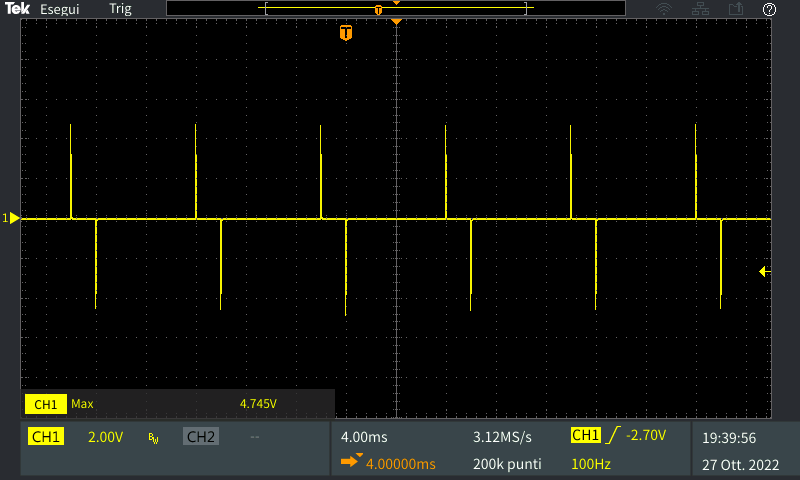
\includegraphics[width=\linewidth]{./ImageFiles/Laboratorio 4/TEK00002.PNG}
	\caption{Misure del segnale $v_{+}$ (linea gialla). Questi picchi sono generati dal circuito derivatore con in ingresso un'onda quadra con \textit{duty-cicle} del 20\%, frequenza di \SI{100}{\hertz} e ampiezza picco-picco pari a \SI{10}{\volt}.}
	\label{fig:picchi_ingresso}
\end{figure}

In figura \ref{fig:segnale_uscita} sono invece mostrati gli andamenti di $v_{-}$ e $v_{out}$. È interessante notare che i valori di saturazione dell'amplificatore operazionale, e quindi i valori tra cui commuta $v_{out}$, sono minori delle tensioni di alimentazione $V_{DD}$ e $V_{SS}$.
\begin{figure}[h!]
	\centering
	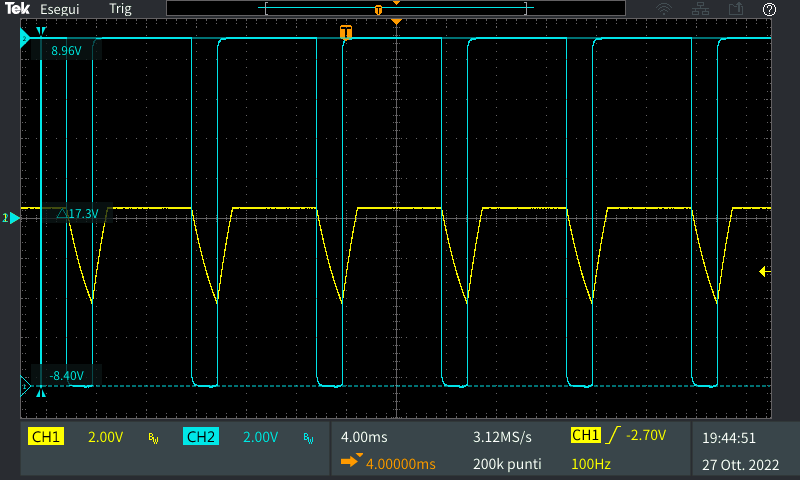
\includegraphics[width=\linewidth]{./ImageFiles/Laboratorio 4/TEK00008.PNG}
	\caption{Misure del segnale $v_{-}$ (linea gialla) e del segnale $v_{out}$ (linea azzurra).}
	\label{fig:segnale_uscita}
\end{figure}
\todo{Abbiamo una formula con cui calcolare il tempo di scarica e confrontarlo con quello che abbiamo in una delle imagini?}
\todo{Scriviamo che con il ua741 non funzionava?}
\newpage
Il secondo circuito visto a lezione è una variante del circuito precedente implementata tramite un integrato 555 al posto di un amplificatore operazionale. Di seguito il circuito costruito.\todo{Circuito e immagine qua}.

L'integrato 555 è composto da diversi componenti al suo interno, collegati ai suoi piedini esterni:
\begin{figure}[h!]
	\centering
	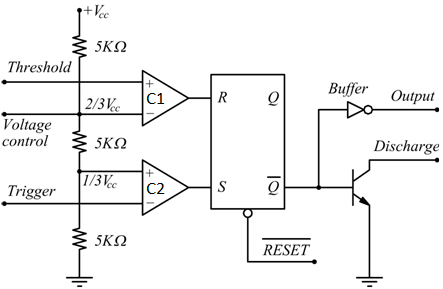
\includegraphics[width=\linewidth]{./ImageFiles/Laboratorio 4/555internals.jpg}
	\caption{Struttura interna di un circuito integrato 555}
	\label{fig:555_internals}
\end{figure}

\noindent
Quando il generatore di segnale collegato tra il pin 2 e la massa del circuito 555 rimane alta, questo risulta sempre $>=\frac{1}{3}V_{CC}$, che quindi mantiene il secondo comparatore con un uscita bassa. Ipotizzando che il suo stato iniziale non sia settato il flip flop mantiene lo stato basso in uscita, e la sua uscita negata risulta alta. Ciò mantiene chiuso l'interruttore che collega a massa il pin 6 e la capacità, mantenendo quindi il circuito in questo stato fino a quando lo stato sul pin 2 non commuta ad uno stato basso.

\noindent
Quando ciò avviene, il morsetto del secondo comparatore risulta più negativo di $\frac{1}{3}V_{CC}$, che quindi fa commutare il comparatore e il flip flop cambia stato portando l'uscita ad uno stato alto. Questo quindi causa l'apertura dell'interruttore sul piedino 7 e la capacità ora può iniziare a caricarsi lentamente tramite la resistenza $R$ messa tra il condensatore e $V_{CC}$. Idealmente questo continuerebbe a caricarsi fino a raggiungere una tensione pari a $V_{CC}$, ma uno dei suoi capi è collegato al primo comparatore, che è collegato ad una tensione di riferimento di $\frac{2}{3}V_{CC}$ sul suo morsetto negativo. Quando quindi il morsetto positivo supera questa soglia, il comparatore imposterà la sua uscita ad un livello alto, resettando quindi il flip flop. Ciò riporterà la sua uscita ad un livello basso, l'interruttore verrà nuovamente chiuso e la capacità verrà cortocircuitata, riportando il circuito allo stato iniziale.

\noindent
Il periodo di carica e scarica varia in base ai valori di $R$ e di $C$, seguendo la relazione
\[v_C = V_{CC}\cdot\left(1-e^{-\frac{t}{RC}}\right)\]
La carica della capacità termina quando $v_C = \frac{2}{3}V_{CC}$, quindi
\[\frac{2}{3}V_{CC} = V_{CC}\cdot\left(1-e^{-\frac{T}{RC}}\right)\]
\[T=-RC\ln\left(\frac{1}{3}\right)\approx1.1RC\]

Per caratterizzare questo circuito abbiamo quindi provato a sostituire valori di $R$ e di $C$ per verificare la legge scritta sopra. Nella tabella \ref{tab:valori_componenti_2} sono indicati i valori che abbiamo scelto.

\def\arraystretch{1.3}
\begin{table}[h]
	\centering
	\begin{tabular}{|c|c|c|}
		\hline
		Componente	& Valore Nominale & Valore Misurato \\ \hline
		R1 &\SI{10}{\kilo\ohm} & \SI{10,96}{\kilo\ohm} \\ \hline
		R2 &\SI{18}{\kilo\ohm} & \SI{18,02}{\kilo\ohm} \\ \hline
		R3 & \SI{12}{\kilo\ohm} & \SI{11,96}{\kilo\ohm} \\ \hline
		R4 & ? & ? \\ \hline
		C1 & \SI{150}{\nano\farad} & Non misurato \\ \hline
		C2 & \SI{330}{\nano\farad} & Non misurato \\ \hline
	\end{tabular}
	\caption{Valori nominali e misurati dei componenti utilizzati nel circuito.}
	\label{tab:valori_componenti_2}
\end{table}
\todo{Completare l'ultimo valore di R usato}
Il segnale in ingresso utilizzato è un'onda quadra con \textit{duty-cicle} pari al 80\%, frequenza di \SI{100}{\hertz} e ampiezza picco-picco pari a \SI{10}{\volt}, con un offset di \SI{5}{\volt}.
\todo{Immagini e grafico di matlab risultante da aggiungere}
